\chapter{Axiomatique et calcul des probabilités}
\section{Introduction}

\section*{Introduction aux Probabilités}

Les probabilités constituent un domaine des mathématiques visant à modéliser et quantifier l'incertitude inhérente à certains phénomènes, qu'ils soient naturels, expérimentaux ou abstraits. Intuitivement, on cherche à associer à chaque \og événement possible \fg{} un nombre compris entre $0$ et $1$ reflétant notre degré de confiance en sa réalisation.

\medskip 

Formaliser rigoureusement cette idée n'est cependant pas immédiat : la théorie moderne des probabilités repose sur la \textbf{théorie de la mesure} et des résultats analytiques qui n'ont pas encore été vus. Un traitement pleinement rigoureux exigerait donc de maîtriser l'\textbf{intégrale de Lebesgue} et la théorie de la mesure, outils qui dépassent le cadre de ce cours. 

\medskip

C'est pourquoi nous adopterons ici une approche volontairement informelle : nous travaillerons principalement sur des espaces de probabilité discrets ou continus simples, en admettant certains résultats analytiques sous-jacents, tout en conservant la rigueur propre aux mathématiques dans les définitions, les énoncés et les démonstrations.

Nous allons alors introduire la notion suivante :

\begin{definition}
    Une \emph{expérience aléatoire} est une expérience dont on connaît l'ensemble des résultats possibles, mais dont le résultat effectif dépend du hasard.
\end{definition}

\begin{notation}
    On note $\Omega$ l'ensemble des résultats possibles de l'expérience aléatoire.
\end{notation}

\begin{exemple} 
    Voici quelques exemples d'expériences aléatoires et de l'ensemble $\Omega$ associé :
    \begin{itemize}
        \item Lancer d'un dé : $\Omega=\{1,2,3,4,5,6\}$. \label{ex:lancer_de}
        \item Lancer de deux pièces : $\Omega= \{(P,P),(P,F),(F,P),(F,F)\}$.
        \item Durée de vie d'une machine : $\Omega = [0,+\infty[$.
    \end{itemize} 
\end{exemple}

\begin{definition}
    Un \emph{événement} est un sous-ensemble des résultats possibles, dont on veut mesurer les chances de réalisation.
\end{definition}

Par exemple, dans le lancer d'un dé (cf. exemple \ref{ex:lancer_de}), on peut définir les événements suivants : $A= \{4\}$ (le résultat est 4), $B= \{1,2,3,4\}$ (le résultat est inférieur ou égal à 4) et $C= \{2,4,6\}$ (le résultat est pair).

\begin{definition}
    On appelle \emph{résultat} (ou issue) le choix d'un élément $\omega\in\Omega$. On dit qu'un événement $A$ est \emph{réalisé} si le résultat $\omega$ appartient à $A$.
\end{definition}

\begin{definition}[approche intuitive]
    Une \emph{mesure de probabilité} est une application 
    \[
    \fonction{P}{\mathcal{A}\to [0,1]}{A \in \partie (A)}
    \]
    où $P(A)$ représente la vraisemblance (ou la chance) que l'événement $A$ se réalise lors de l'expérience, et où $\mathcal{A}$ est l'ensemble des événements.
\end{definition}

Informellement, on interprète $P(A)= 1$ comme le fait que $A$ est certain de se réaliser. Si $P(A)=0$, nous sommes certains que $A$ ne se réalisera pas. Enfin, $P(A)= 0{,}37$ signifie que l'événement $A$ a $37\,\%$ de chances de se réaliser.

Pour calculer $P(A)$, on peut imaginer réaliser $N$ fois l'expérience aléatoire (de manière indépendante) et noter $P_N(A) = \frac{\#\{\text{fois où } A \text{ s'est réalisé}\}}{N}$. On définit alors naïvement la probabilité par passage à la limite :
\[
P(A)= \lim_{N\to +\infty}P_N(A).
\]

\begin{proposition}
    Si $\Omega$ est un ensemble fini et que tous les résultats sont équiprobables, alors :
    \[
    \forall A\in \mathcal{A} \quad P(A) = \frac{\# A}{\#\Omega}.
    \]
\end{proposition}

\begin{remarque}
    Soient $A$ et $B$ des événements. On est souvent amené à considérer les événements composés suivants :
    \begin{itemize}
        \item $A\cup B$ : [$A$ se réalise ou $B$ se réalise] ;
        \item $A\cap B$ : [$A$ se réalise et $B$ se réalise] ;
        \item $A^c$ : [$A$ ne se réalise pas].
    \end{itemize}
\end{remarque}

Il est clair au vu de cette première approche des probabilités d'événements équiprobables que, en pratique, la notion de dénombrement est essentielle. Nous allons voir, dans la section suivante, des outils fort pratiques pour dénombrer un ensemble.

\section{Combinatoire}

L’analyse combinatoire est l’art de compter les éléments d’ensembles finis. Elle est donc cruciale pour calculer des probabilités dans le cas d’équiprobabilité.

\begin{proposition}[Principe fondamental du dénombrement]
    Si l'on considère $k$ expériences $E_1,\dotsc,E_k$ telles que chaque expérience $E_j$ possède $r_j$ résultats possibles, alors le nombre total de résultats possibles pour la suite d'expériences $(E_1,\dots,E_k)$ est donné par le produit $r_1 \cdot r_2 \dotsm r_k$.
\end{proposition}

Le résultat s’effectue sans difficulté par récurrence.

 \begin{exemple}
     Si une personne possède $3$ pulls, $2$ pantalons et $10$ paires de chaussettes, elle a $3\cdot 2\cdot 10 = 60$ façons différentes de s'habiller.
 \end{exemple}  

 
 \begin{definition}  
     Pour tout entier $n\in \N$, on pose $n! = \prod_{i=1}^{n}i$ (avec la convention $0! = 1$). De plus, le cardinal de l'ensemble des permutations $S_n$ d'un ensemble à $n$ éléments (par exemple $\{1,\dotsc,n\}$) vaut $S_n = n!$.
 \end{definition}

 \begin{notation}
     Pour $n, k \in \N$ avec $k\le n$, on définit le coefficient binomial par :
     \[
     \binom{n}{k} := \frac{n!}{k!(n-k)!}.
     \]
 \end{notation}

 \begin{proposition}
     Le coefficient $\binom{n}{k}$ représente le nombre de sous-ensembles à $k$ éléments que l'on peut former à partir d'un ensemble à $n$ éléments.
 \end{proposition}

 \begin{proof}
    À partir de $n$ éléments distincts, on souhaite former un vecteur constitué de $k$ éléments distincts. Pour la première composante, on a $n$ possibilités ; pour la deuxième, on en a $n-1$ ; et pour la $i$-ème, on a $n-i+1$ possibilités. 
    Par le principe du dénombrement, il y a donc $n(n-1)(n-2)\dotsm(n-k+1)$ tels vecteurs. 
    
    Néanmoins, ce nombre ne correspond pas au nombre de sous-ensembles à $k$ éléments, car dans un ensemble, l'ordre des éléments n'a pas d'importance. À chaque sous-ensemble de $k$ éléments, on peut associer exactement $k!$ vecteurs correspondants (ses permutations). Ainsi, le résultat attendu est obtenu en divisant par $k!$ :
    \[
    \frac{n(n-1)\dotsm(n-k+1)}{k!} = \binom{n}{k}.
    \]
 \end{proof}

\begin{remarque}
    Certains problèmes de combinatoire peuvent se résoudre en utilisant ce principe et (d'autres) formulé de manière intuitive. En effet, pour des soucis de lourdeur d'écriture il n'est pas toujours nécessaire d'écrire explicitement les bijection entre des ensembles fini.
\end{remarque}

\begin{proposition}
    Les égalités suivantes sont vérifiées :
    \begin{itemize}
        \item $\displaystyle \binom{n}{k} = \binom{n}{n-k}$
        \item $\displaystyle \sum_{k = 0}^n \binom{n}{k} = 2^n$
    \end{itemize}
\end{proposition}

\begin{proof}
    \begin{itemize}
        \item À chaque sous-ensemble de $k$ éléments, on peut faire correspondre de manière bijective un et un seul sous-ensemble de $n-k$ éléments : son complémentaire.
        \item Le nombre total de sous-ensembles d'un ensemble à $n$ éléments (l'ensemble des parties $\mathcal{P}(\Omega)$) est $2^n$. Partitionner cet ensemble selon la taille $k$ des sous-ensembles donne bien la somme des coefficients binomiaux. 
    \end{itemize}
\end{proof}

\begin{proposition}[Modèles d'urnes]
    Supposons que l'on dispose de $k$ boules et de $n$ urnes numérotées. Le nombre de façons de répartir les $k$ boules dans les $n$ urnes est donné par le tableau suivant :
    \begin{center}
    \renewcommand{\arraystretch}{1.8}
    \begin{tabular}{|c|c|c|}
         \hline
         & \textbf{Boules identiques} & \textbf{Boules discernables} \\
         \hline
         \textbf{Max. 1 boule par urne} & $\displaystyle \binom{n}{k}$ & $\displaystyle \frac{n!}{(n-k)!}$ \\
         \hline
         \textbf{Pas de contrainte} & $\displaystyle \binom{n+k-1}{k}$ & $n^k$ \\
         \hline
    \end{tabular}
    \end{center}
\end{proposition}

\begin{proof}
    Démontrons chacun des 4 cas :
    \begin{enumerate}
        \item \textbf{Max 1 boule, identiques :} Il s'agit simplement de choisir $k$ urnes parmi $n$. Soit $\binom{n}{k}$ choix.
        \item \textbf{Max 1 boule, discernables :} On choisit la $1^{\text{ère}}$ urne parmi $n$, la $2^{\text{ème}}$ parmi $n-1$, etc. Soit $n(n-1)\dotsm(n-k+1)$ choix.
        \item \textbf{Sans contrainte, identiques :} Voyons les boules comme des points et les séparations entre les urnes comme des parois. À chaque configuration, on associe une suite constituée de $k$ boules et de $n-1$ parois intérieures. Cela équivaut à choisir l'emplacement des $k$ boules parmi $n+k-1$ positions totales. Ainsi, on obtient $\binom{n+k-1}{k}$ possibilités.
        \item \textbf{Sans contrainte, discernables :} Chaque boule peut être placée librement dans l'une des $n$ urnes. Pour $k$ boules, cela donne $n^k$ possibilités.
    \end{enumerate}
\end{proof}

\begin{exemple}
    Supposons avoir $k$ boules identiques et $n$ urnes. On cherche le nombre de façons de répartir les boules de sorte que l'urne $j$ contienne au moins $c_j$ boules. En posant $c= \sum_{j=1}^n c_j$, on commence par placer ces $c$ boules. Il reste alors $k-c$ boules à répartir sans contrainte dans les $n$ urnes. D'après le troisième modèle d'urnes, on obtient $\binom{n+(k-c)-1}{k-c}$ possibilités.
\end{exemple}

\begin{exemple}
    Supposons avoir $l$ boules rouges et $k$ boules noires (identiques entre elles) à placer dans $n$ urnes (avec $n\ge l+k$), à raison d'au maximum une boule par urne. Par le principe du dénombrement, on choisit d'abord les $k$ urnes pour les boules noires ($\binom{n}{k}$ choix), puis $l$ urnes parmi les $n-k$ restantes pour les rouges ($\binom{n-k}{l}$ choix). Soit $\binom{n}{k} \binom{n-k}{l}$ possibilités.
\end{exemple}

\begin{exemple}
    Combien y a-t-il de solutions dans $\N^n$ à l'équation : $x_1 + x_2 + \dotsb + x_n = k$ ?\\
    Il s'agit exactement du nombre de façons de répartir $k$ unités (boules identiques) dans $n$ variables (urnes), sans contrainte. La solution est donc $\binom{n+k-1}{k}$.
\end{exemple}

\begin{proposition}[Identité de Pascal]
    Soit $n\in \N_0$ et $0<k<n$. On a :
    \[
    \binom{n}{k} = \binom{n-1}{k} + \binom{n-1}{k-1}
    \]  
\end{proposition}

\begin{proof}
    Soit $A \subseteq \{1,\dotsc, n\}$ un sous-ensemble possédant $k$ éléments. 
    \begin{itemize}
        \item Si $n \in A$, alors $A = A'\sqcup \{n\}$ où $A' \subseteq \{1,\dotsc,n-1\}$ contient $k-1$ éléments. Il y a $\binom{n-1}{k-1}$ tels sous-ensembles.
        \item Si $n \notin A$, alors $A \subseteq \{1,\dotsc, n-1\}$ et contient $k$ éléments. Il y a $\binom{n-1}{k}$ tels sous-ensembles.
    \end{itemize}
    La somme de ces deux cas exclusifs donne le résultat.
\end{proof}

\begin{definition}[Triangle de Pascal]
    Le triangle de Pascal obéit aux règles de construction suivantes :
    \begin{itemize}
        \item La première ligne commence par un sommet contenant $1$.
        \item On construit chaque nouvelle case en faisant la somme des deux coefficients situés directement au-dessus d'elle (à gauche et à droite).
    \end{itemize}
    Remarquons que si $k = 0$ ou $k= n$, on a $\binom{n}{k} = 1$. Par l'identité de Pascal, ce triangle contient exactement les coefficients binomiaux.
\end{definition}

\begin{figure}[htbp]
    \centering
    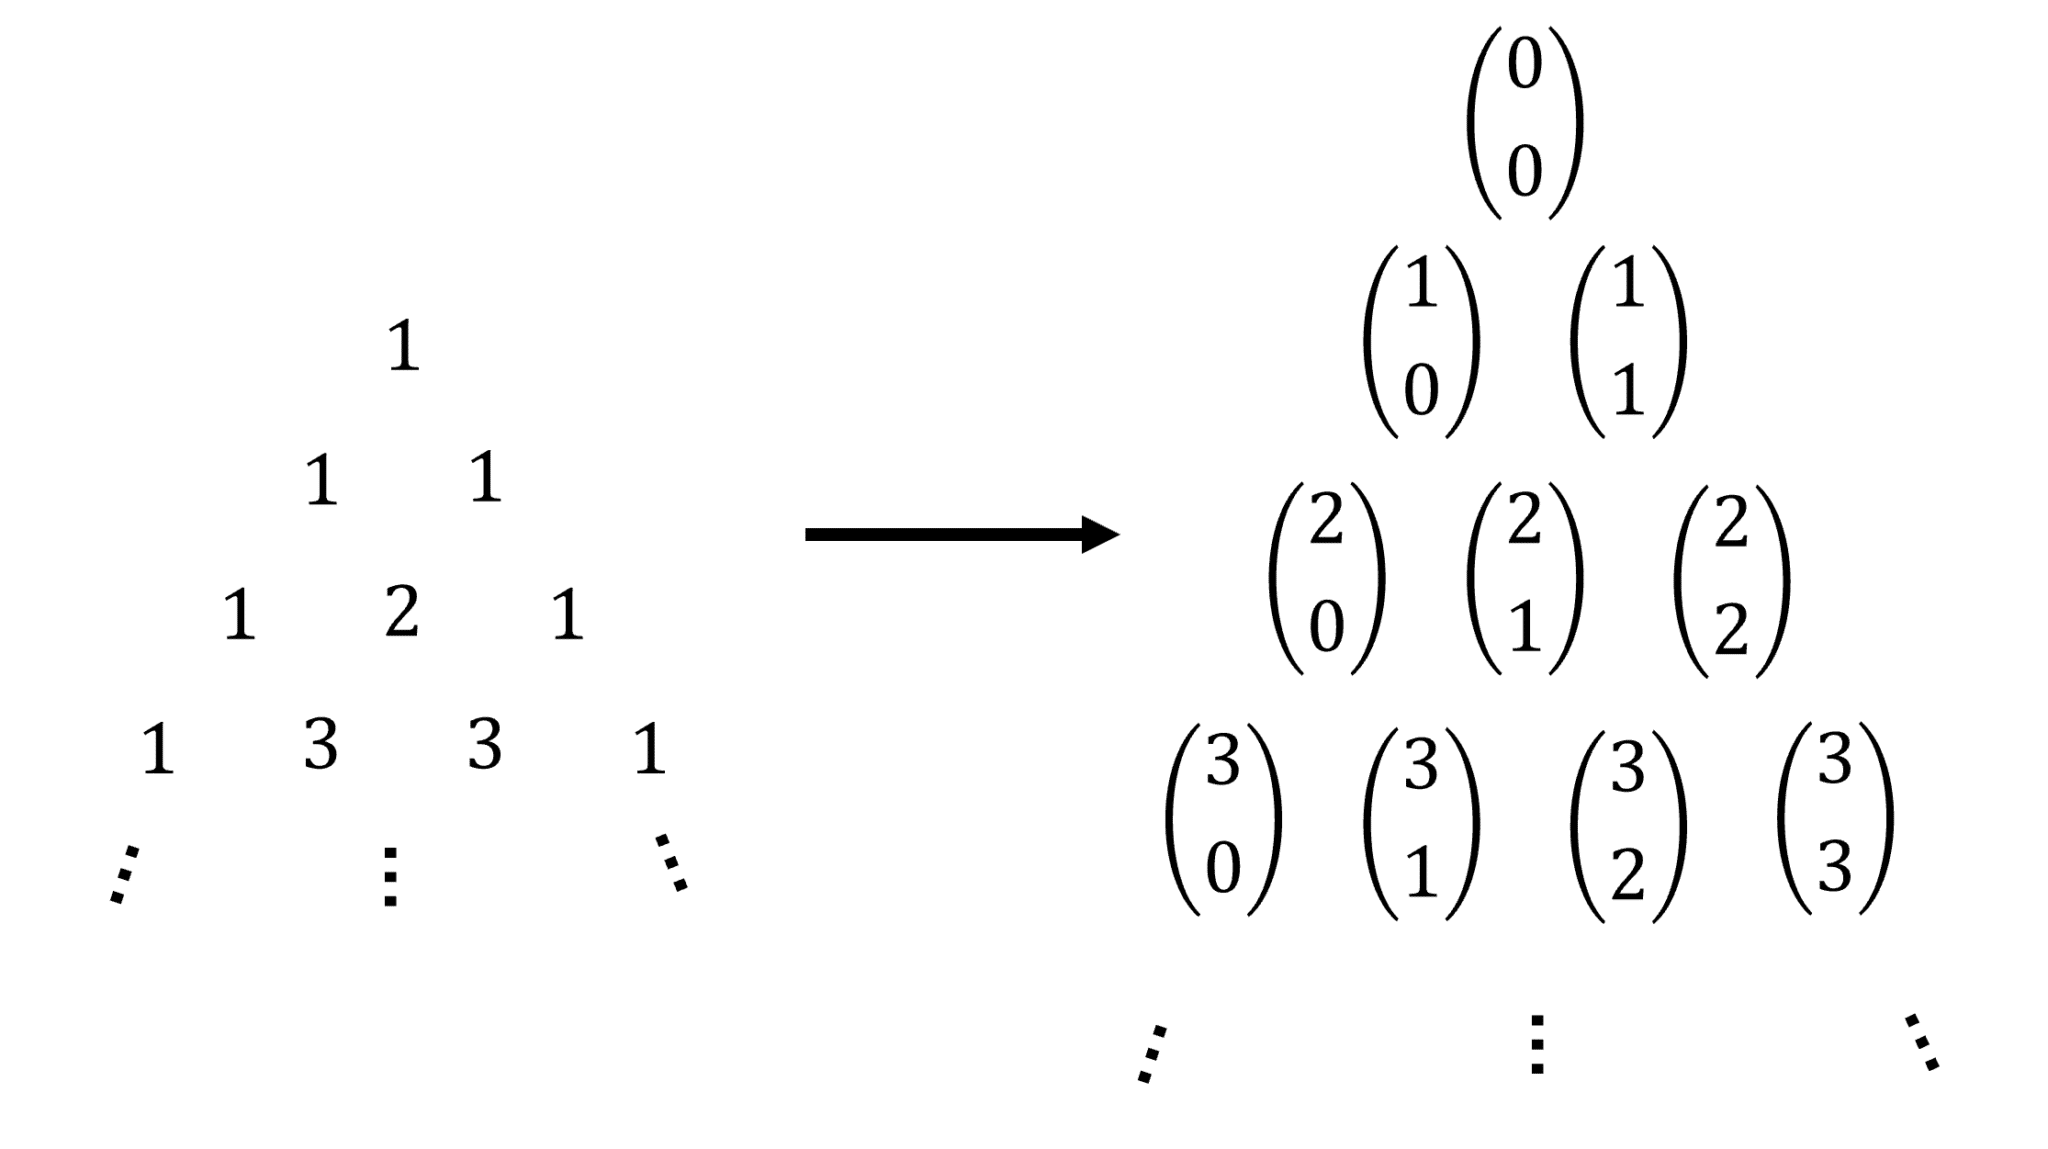
\includegraphics[width=0.5\linewidth]{imageyo.png}
    \caption{Triangle de Pascal}
    \label{fig:pascal}
\end{figure}

\begin{proposition}[Binôme de Newton]
   Soient $A$ un anneau et $a,b\in A$ tels que $ab= ba$ (ils commutent). Pour tout entier naturel $n$, on a :
   \[
   (a+b)^n = \sum_{k = 0}^n \binom{n}{k} a^k b^{n-k}
   \] 
\end{proposition}

\begin{exemple}[Équation de récurrence]
    On souhaite construire une guirlande composée de $n \ge 1$ boules. Pour ce faire, nous disposons de trois types différents de morceaux de guirlandes. Le premier est composé de deux boules bleues, le second de trois boules jaunes et le dernier de cinq boules rouges. 
    
    En notant $X_n$ le nombre de possibilités, on trouve facilement les premières valeurs : $X_1= 0$, $X_2 = 1$, $X_3=1$, $X_4=1$ et $X_5=3$. On en déduit l'équation de récurrence linéaire suivante :
    \[
  \forall n\ge 6, \quad  X_n=X_{n-2}+X_{n-3}+X_{n-5} 
    \]
    Pour la résoudre, on passe sous forme matricielle. Dès lors, on pose :
    \[
    Y_n = \begin{pmatrix}
        X_n \\ X_{n-1} \\ X_{n-2} \\ X_{n-3} \\ X_{n-4}
    \end{pmatrix}
    = \begin{pmatrix}
        0 & 1 & 1 & 0 & 1 \\
        1 & 0 & 0 & 0 & 0 \\
        0 & 1 & 0 & 0 & 0 \\
        0 & 0 & 1 & 0 & 0 \\
        0 & 0 & 0 & 1 & 0 \\
    \end{pmatrix}
    \begin{pmatrix}
        X_{n-1} \\ X_{n-2} \\ X_{n-3} \\ X_{n-4} \\ X_{n-5}
    \end{pmatrix}
    = M Y_{n-1}
    \]
    Ainsi, nous devons résoudre $Y_n = M Y_{n-1} = M^2 Y_{n-2} = \dots = M^{n-5} Y_5$. La solution générale s'écrit donc :
    \[
    Y_n = M^{n-5} Y_5 = M^{n-5} 
    \begin{pmatrix}
        3 \\ 1 \\ 1 \\ 1 \\ 0
    \end{pmatrix}
    \]
\end{exemple}

\begin{exemple}[Paradoxe des anniversaires]
    Considérons une pièce contenant $n \le 365$ personnes. Quelle est la probabilité qu'au moins deux de ces personnes aient la même date d'anniversaire ?
    
    On fait les hypothèses suivantes : l'année compte $365$ jours, et la date d'anniversaire de chaque personne est distribuée uniformément au hasard indépendamment des autres. Soit $A = [\text{au moins deux personnes partagent leur anniversaire}]$. Il est plus simple de calculer la probabilité de l'événement complémentaire $A^c = [\text{toutes les personnes ont des anniversaires différents}]$. On a :
    \begin{align*}
        P(A) &= 1 - P(A^c) \\
        &= 1 - \frac{\# A^c \text{ (cas favorables à } A^c)}{\# \Omega \text{ (tous les cas possibles)}}
    \end{align*}
    En utilisant l'analogie des urnes (on place $n$ boules discernables dans $365$ urnes), on déduit que le nombre de cas possibles sans contrainte est $365^n$. Le nombre de cas favorables à $A^c$ (au maximum une boule par urne) est $\frac{365!}{(365-n)!}$. On trouve alors :
    \[
    P(A) = 1 - \frac{365!}{365^n (365-n)!}
    \]
    Voici quelques valeurs remarquables :
    \begin{center}
    \begin{tabular}{|c|c|}
       \hline
       \textbf{Nombre de personnes} ($n$) & $\boldsymbol{P(\exists \text{ anniversaire commun})}$ \\
       \hline
       5  & $0{,}027$ \\
       15 & $0{,}253$ \\
       23 & $0{,}507$ \\
       30 & $0{,}706$ \\
       50 & $0{,}970$ \\
       70 & $0{,}999$ \\
       \hline
    \end{tabular}
    \end{center}
    \textit{Remarque : Dès 23 personnes, il y a plus de 50\,\% de chances que deux d'entre elles partagent la même date d'anniversaire.}
\end{exemple}

Cette première approche intuitive des probabilités consiste à considérer un ensemble d’événements dont on veut déterminer les chances de réalisation et y associé un nombre entre $0$ et $1$ avec l'interprétation qu'on lui a prêté plus haut. Cette approche s'avère très inintéressante pour déterminer les axiomes qui amèneront les "bonnes" propriétés intuitives qu'on espère avoir pour modéliser cette idée.


\section{Axiomatique des probabilités}



\begin{definition}
    Un \emph{espace de probabilités} est un triplet $(\Omega, \mathscr A, P)$ tel que :
    \begin{itemize}
        \item $\Omega$ est un ensemble quelconque.
        \item $\mathscr A$ est une $\sigma$-algèbre sur $\Omega$, \textit{i.e.} $\mathscr A\subseteq \partie(\Omega)$ et vérifie :
        \begin{enumerate}
            \item $\Omega\in\mathscr A$
            \item $A\in\mathscr A \alors A^c\in\mathscr A$
            \item $\displaystyle A_1,A_2,\dotsc\in\mathscr A \alors \bigcup_{n=1}^\infty A_n\in\mathscr A$
        \end{enumerate}
        \item $P$ est une mesure de probabilité, c'est-à-dire une application $P: \mathscr A \to [0,1]$ telle que :
        \begin{enumerate}
            \item $P(\Omega)=1$
            \item $P$ est $\sigma$-additive, c'est-à-dire que pour $A_1,A_2,\dots\in \mathscr A$ disjoints deux à deux ($A_i\cap A_j= \varnothing$ si $i\neq j$) :
            \[
            P\left(\bigsqcup_{n=1}^{\infty}A_n\right) = \sum_{n=1}^{\infty}P(A_n)
            \]
        \end{enumerate}
    \end{itemize}
    
    Intuitivement :
    \begin{itemize}
        \item $\Omega = \{\text{résultats possibles de l'expérience}\}$, et donc une expérience est le choix d'un $\omega\in\Omega$ (avec l'intervention du hasard).
        \item \begin{align*}
            \mathscr A &= \text{« l'ensemble des événements »}\\
            &= \text{« l'ensemble des observations que l'on sera en mesure de faire sur le résultat}\\
            &\quad \text{de l'expérience aléatoire »}
        \end{align*}
        \item \begin{align*}
            P(A) &= \text{« la mesure de probabilité de $A\in\A$ »} = \text{« la probabilité de $A$ »}\\
            &= \text{« la chance que l'événement $A$ se produise au cours de l'expérience aléatoire,}\\
            &\quad \text{ ie $\omega\in A$ »}
        \end{align*}
    \end{itemize}
\end{definition}

A présent, constatons les conséquences de cette axiomatique.

\begin{proposition}
    Soit $\mathscr A$ une $\sigma$-algèbre sur $\Omega$. Alors :
    \begin{enumerate}
        \item $\varnothing \in \mathscr A$
        \item $A_1,A_2,\dots \in \mathscr A \alors \bigcap_{n=1}^{\infty} A_n \in \mathscr A$ 
        \item $A,B\in \mathscr A \alors A\cup B\in \mathscr A,\ A\cap B \in \mathscr A,\ A\setminus B \in \mathscr A,\ A\setminus B\in \mathscr A$
    \end{enumerate}
\end{proposition}

\begin{proof}
    \begin{enumerate}
        \item $\varnothing = \Omega^c \in \A$.
        \item De $A_1,A_2,\dotsc\in\A$, on déduit $A_1^c,A_2^c,\dotsc\in\A$, d'où $\bigcup_{n=1}^\infty A_n^c\in\A$. Par les lois de De Morgan, $\bigcap_{n=1}^\infty A_n = \left(\bigcup_{n=1}^\infty A^c_n\right)^c\in\A$.
        \item Soient $A,B\in \A$. On a $A\cup B= \bigcup_{i=1}^\infty A_i$ où $A_1=A$, $A_2=B$ et $A_n= \varnothing$ si $n\ge 3$. De même, on montre que $A\cap B\in\A$. On a ensuite $A\setminus B = A\cap B^c \in \A$. Enfin, $A\setminus B = (A\setminus B)\cup (B\setminus A) \in \A$.
    \end{enumerate}
\end{proof}

Une $\sigma$-algèbre est donc un ensemble fermé par les opérations ensemblistes, ce qui est fort pratique.

\begin{proposition}
    Soit $P$ une mesure de probabilité sur $(\Omega, \A)$ :
    \begin{enumerate}
        \item $P(A\sqcup B) = P(A)+P(B)$
        \item $P(\varnothing)=0$
        \item $A,B\in \mathscr A, A\subseteq B \alors P(A) \leq P(B)$
        \item $A\in \A \alors P(A^c)= 1- P(A)$
        \item $A,B\in \A \alors P(A\cup B)= P(A)+P(B)-P(A\cap B)$
        \item $P(A\setminus B)= P(A)- P(A\cap B)$
    \end{enumerate}
\end{proposition}

\begin{proof}
    \begin{enumerate}
        \item Découle de la $\sigma$-additivité avec $A_1=A$, $A_2=B$ et $A_n=\varnothing$ pour $n \ge 3$.
        \item $P(\varnothing) = P(\varnothing \sqcup \varnothing) = P(\varnothing) + P(\varnothing) \alors P(\varnothing) = 0$.
        \item $B=A\sqcup (B\setminus A)\alors P(B)= P(A)+ P(B\setminus A)\alors P(B) \ge P(A)$ (car $P \ge 0$).
        \item $1 = P(\Omega) = P(A\sqcup A^c) = P(A)+P(A^c)$.
        \item $A\cup B= A\sqcup (B\cap A^c)\alors P(A\cup B)= P(A) + P(B\cap A^c)$. Or, $B = (B\cap A) \sqcup (B\cap A^c)$, d'où $P(B) = P(A\cap B) + P(B\cap A^c)$. En remplaçant, on obtient l'égalité voulue.
        \item $A = (A\setminus B)\sqcup(A\cap B)\alors P(A) = P(A\setminus B) + P(A\cap B)$.
    \end{enumerate}
\end{proof}

Ces propriétés sont forts naturels et souhaitable. Pour s'en rendre compte il suffit que considérer une diagramme de Venn.

\begin{exemple}[Lancer d'un dé]
    On prend $\Omega = \{1,2,3,4,5,6\}$, $\A = \partie(\Omega)$ et :
    \[
    \fonction{P}{\A\to\interff{0,1}}{A\to P(A) = \frac{\# A}{6}}
    \]
\end{exemple}

\begin{proposition}[Inégalité de Boole]
    Soient $(\Omega,\A, P)$ un espace probabiliste et $A_1,A_2,\dots \in \A$.
    \[
    P\left(\bigcup_{n=1}^{\infty}A_n\right)\leq \sum_{n=1}^\infty P(A_n)
    \]
\end{proposition}

\begin{proof}
    On définit par récurrence $B_1 = A_1$ et $B_n = A_n\setminus \bigcup_{i = 1}^{n-1}A_i$ pour $n > 1$. On a $\bigsqcup_{n=1}^\infty B_n = \bigcup_{n=1}^\infty A_n$, d'où :
    \[
    P\left(\bigcup_{n = 1}^\infty A_n\right) = P\left(\bigsqcup_{n = 1}^\infty B_n\right) = \sum_{n = 1}^\infty P(B_n) \le \sum_{n = 1}^\infty P(A_n)
    \]
    car $P(B_n)\le P(A_n)$ vu que $B_n\subseteq A_n$.
\end{proof}

\begin{proposition}[Principe d'inclusion-exclusion]
    Soient $(\Omega,\A, P)$ un espace probabiliste et $A_1,A_2,\dots, A_n \in \A$. On a :
    \[
    P\left(\bigcup_{i=1}^n A_i \right)= \sum_{k=1}^n (-1)^{k+1}\left( \sum_{1\leq i_1<\dots<i_k\leq n} P\left(\bigcap_{j=1}^k A_{i_j}\right)\right)
    \]
\end{proposition}

\begin{proof}
    La démonstration se fait par récurrence sur $n$, en utilisant l'égalité $P(A\cup B) = P(A)+P(B) - P(A\cap B)$.
\end{proof}

\section{Probabilités conditionnelles et indépendance}

\begin{definition}
    Soient $(\Omega,\A, P)$ un espace probabiliste et $A,B\in \A$ avec $P(B)\neq 0$.
    La probabilité conditionnelle de $A$ sachant $B$ est définie par :
    \[
    P(A\mid B)=\frac{P(A\cap B)}{P(B)}
    \]
    On dit que $P(A\mid B)$ est la probabilité de $A$ sachant $B$.
\end{definition}

\begin{remarque}
    Afin d'éviter d'avoir à supposer que $P(B) \neq 0$, on peut utiliser la forme multiplicative : $P(A\cap B) = P(A\mid B)P(B)$.
\end{remarque}
   
Intuitivement la probabilité de $A$ sachant $B$ est la probabilité que la "fraction" de $A$ qui se réalise lorsque $B$ est réalisé.

\begin{exemple}[Lancer d'un dé]
    $A=[\text{le résultat est 4}]$, $B=[\text{le résultat est pair}]$. 
    Ici, $P(A\mid B)= \frac{P(A\cap B)}{P(B)} = \frac{P(A)}{P(B)}= \frac{1/6}{1/2} = \frac{1}{3}$.
\end{exemple}

\begin{remarque}
    L'application 
    \[
    \fonction{P_B}{\A}{\interff{0}{1}}{A}{P_B(A) = P(A\mid B)}
    \]
    est une mesure de probabilité. Toutes les propriétés des mesures de probabilité restent donc vraies pour $P_B$.
\end{remarque}

\begin{exercice}[Événement certain]
    Montrer que si $P(A)=1$, alors pour tout événement $B$ tel que $P(B)>0$, on a $P(A\mid B)=1$.
\end{exercice}

\begin{theoreme}[Probabilités totales]
    Soient $(\Omega,\A, P)$ un espace probabiliste et $\{B_n\}$ une partition finie ou dénombrable de $\Omega$ vérifiant $\forall n,\ B_n\in \A$ et $P(B_n)>0$. Alors :
    \[
    P(A) = \sum_n P(A\mid B_n)P(B_n)
    \]
\end{theoreme}

\begin{proof}
    Nous avons que :
    \begin{align*}
        P(A) &= P(A\cap \Omega)\\
        &= P\left(A\cap \left(\bigsqcup_n B_n\right)\right)\\ 
        &= \sum_{n} P(A\cap B_n)\\ 
        &= \sum_n P(A\mid B_n)P(B_n)
    \end{align*}  
\end{proof}



\begin{exemple}
    Supposons qu'il n'y ait que deux temps possibles demain :
    \begin{itemize}
        \item Pas beau : $20\%$ de chances que je sorte.
        \item Beau : $70\%$ de chances que je sorte.
    \end{itemize}
    Quelle est la probabilité que je sorte demain, sachant que la météo m'informe qu'il y a $40\%$ de chances de mauvais temps ?
    \[
    P(\text{sors}) = P(\text{sors}\mid \text{beau})P(\text{beau}) + P(\text{sors}\mid \text{pas beau})P(\text{pas beau}) = 0{,}7\cdot 0{,}6 + 0{,}2\cdot 0{,}4 = 0{,}5
    \]
\end{exemple}

\begin{proposition}[Règle de Bayes]
    Soient $(\Omega,\A, P)$ un espace probabiliste et $A,B\in \A$ avec $P(B)\neq 0$. Nous avons que :
    \[
    P(A\mid B)= \frac{P(B\mid A)P(A)}{P(B)}
    \]
\end{proposition}

\begin{proof}
    Nous avons que :
    \begin{align*}
       P(A\mid B) &= \frac{P(A\cap B)}{P(B)} \\
       &= \frac{P(B\cap A)}{P(B)} \\
       &= \frac{P(B\mid A)P(A)}{P(B)}
    \end{align*}   
\end{proof}

\begin{exemple}[Paradoxe du faux positif]
    Une infection mortelle (le covid-10000) se propage dans une population, et on dispose d'un test PCR. Le vendeur nous indique que :
    \begin{itemize}
        \item Il y a $95\%$ de chances que le test soit positif si la personne testée est infectée.
        \item Il y a $1\%$ de chances de faux positifs (test positif alors que la personne est saine).
        \item $0{,}5\%$ de la population est infectée.
    \end{itemize}
    De plus, un traitement existe, mais il est très risqué ($50\%$ de chances d'être mortel). Si une personne se présente avec un test positif, doit-elle prendre le traitement ?
\end{exemple}

\begin{proof}[Résolution]
    Posons $A = [\text{l'individu est infecté}]$ et $B=[\text{le test est positif}]$. 
    \begin{align*}
        P(A\mid B) &= \frac{P(B\mid A)P(A)}{P(B)}\\ 
        &= \frac{P(B\mid A)P(A)}{P(B\mid A)P(A)+P(B\mid A^c)P(A^c)}\\
        &= \frac{0{,}95\cdot 0{,}005}{0{,}95\cdot 0{,}005 + 0{,}01\cdot 0{,}995} \simeq 0{,}323
    \end{align*}
    La probabilité d'être réellement malade sachant que le test est positif n'est que d'environ $32{,}3\%$. Prendre un traitement mortel dans $50\%$ des cas serait donc déraisonnable. Il y a ici une confusion classique entre $P(A\mid B)$ et $P(B\mid A)$.
\end{proof}

\begin{notation}
    On note souvent $P(A,B)= P(A\cap B)$ et $P(A\mid B,C)= P(A\mid B\cap C)$.
\end{notation}

\begin{definition}[Indépendance]
    Soient $(\Omega, \A,P)$ un espace de probabilités et $A,B\in\A$. On dit que $A$ et $B$ sont indépendants, ce que l'on note $A\indep B$, si $P(A\cap B) = P(A)P(B)$, ou, de façon équivalente (si $P(B)>0$), si $P(A \mid B) = P(A)$.
\end{definition}

\begin{exemple}[Lancer de $2$ pièces]
    On note $A=[\text{la pièce } 1 \text{ tombe sur pile}]$, $B= [\text{la pièce } 2 \text{ tombe sur pile}]$ et $C=[\text{les deux pièces tombent sur pile}]$.
    \begin{itemize}
        \item $A\indep B$ : On a $P(A\cap B) =\frac{1}{4} = \frac{1}{2}\cdot\frac{1}{2} = P(A)P(B)$.
        \item $A\nindep C$ : On a $P(A\cap C) = P(C) = \frac{1}{4}$ mais $P(A)P(C) = \frac{1}{2}\cdot\frac{1}{4} = \frac{1}{8}$.
    \end{itemize}
\end{exemple}

\begin{definition}
    Soient $(\Omega, \A,P)$ un espace de probabilités et $(A_i)_{i\in I}$ une famille d'événements.
    \begin{itemize}
        \item Les $A_i$ sont \emph{indépendants deux à deux} si :
        \[
        \forall i\neq j, \quad A_i \indep A_j 
        \]
        \item Les $A_i$ sont \emph{mutuellement indépendants} (ou indépendants dans leur ensemble) si :
        \[
        \forall J\subseteq I \text{ fini}, \quad P\left(\bigcap_{j\in J}A_j\right)=\prod_{j\in J}P(A_j)
        \]
    \end{itemize}
\end{definition}

\begin{exemple}
    On a $4$ cartes : rouge, verte, bleue et multicolore (contenant les 3 couleurs). On tire une carte au hasard, et on pose $R = [\text{la carte contient du rouge}]$ ; de même pour $B$ et $V$.
    \begin{description}
        \item[$R, B, V$ sont indépendants deux à deux :] On a $P(R\cap B) = \frac{1}{4}$ (seule la carte multicolore contient à la fois du rouge et du bleu). Or, $P(R) = P(B) = P(V) = \frac{2}{4} = \frac{1}{2}$. On a bien $P(R\cap B) = P(R)P(B) = \frac{1}{4}$.
        \item[$R, B, V$ ne sont pas mutuellement indépendants :] On a $P(R\cap B\cap V) = \frac{1}{4}$ (la carte multicolore), ce qui est différent de $P(R)P(B)P(V) = \frac{1}{8}$.
    \end{description}
\end{exemple}

\begin{exemple}[Affaire Sally Clark]
    \begin{itemize}
        \item Il y a environ $0{,}01\%$ de chances qu'un nourrisson meure de mort subite.
        \item L'expert a calculé les chances que les deux enfants meurent de mort subite ainsi : $\frac{1}{10^4} \cdot \frac{1}{10^4} = \frac{1}{10^8} \simeq 0$.
    \end{itemize}
    Ce raisonnement souffre de deux problèmes majeurs :
    \begin{itemize}
        \item L'hypothèse d'indépendance (la génétique ou l'environnement rendent ces événements dépendants).
        \item Il y a eu une confusion entre deux probabilités conditionnelles (le sophisme du procureur). Posons $I = [\text{Sally est innocente}]$ et $M = [\text{les deux enfants meurent en bas âge}]$. L'argument de l'expert porte sur $P(M\mid I)$, or ce qui intéresse la justice est $P(I\mid M)$. Par la formule de Bayes :
        \[
        P(I\mid M ) = \frac{P(M\mid I)P(I)}{P(M\mid I)P(I) + P(M\mid I^c)P(I^c)} \simeq 1
        \]
        vu que $P(I^c)$ (la probabilité a priori qu'une mère soit une double meurtrière) est extrêmement faible, proche de $0$.
    \end{itemize}
\end{exemple}

\section{Suites d'événements, lemme de Borel-Cantelli}

\begin{definition}
    Soient $(\Omega, \A, P)$ un espace de probabilité et $(A_n)$ une suite d'événements dans $\A$.
    \begin{itemize}
        \item Si $(A_n)$ est croissante, ie $(A_n \subseteq A_{n+1})$, on définit sa limite comme :
        \[
        \lim_{n\to +\infty}A_n = \bigcup_{n=1}^{\infty} A_n
        \]
        \item Si $(A_n)$ est décroissante, ie $(A_{n+1} \subseteq A_n)$, on définit sa limite comme :
        \[
        \lim_{n\to +\infty}A_n = \bigcap_{n=1}^{\infty} A_n
        \]
    \end{itemize}
\end{definition}

\begin{theoreme}[Continuité des probabilités]
    Si $(A_n)$ est une suite monotone dans $\A$, alors :
    \[
    \lim_{n\to\infty} P(A_n) = P\left(\lim_{n\to\infty}A_n\right)
    \]
\end{theoreme}

\begin{proof}
    \textbf{Cas où $(A_n)$ est croissante :} On pose $B_1 = A_1$ et $B_k = A_k\setminus A_{k-1}$ pour $k \ge 2$. Les ensembles $B_k$ sont disjoints et on a :
    \[
    \bigsqcup_{n=1}^\infty B_n = \bigcup_{n=1}^\infty A_n
    \]
    Par la $\sigma$-additivité de $P$, on obtient :
    \begin{align*}
        P\left( \bigcup_{n=1}^{\infty}A_n\right) &= P\left(\bigsqcup_{n=1}^{\infty}B_n\right)\\
        &= \sum_{n = 1}^\infty P(B_n) = \lim_{N\to\infty} \sum_{n = 1}^N P(B_n)\\
        &= \lim_{N\to\infty} P\left(\bigsqcup_{n = 1}^N B_n\right) = \lim_{N\to\infty}P(A_N)
    \end{align*}
    
    \textbf{Cas où $(A_n)$ est décroissante :} On considère la suite complémentaire $(A^c_n)$, qui est croissante. Par les lois de De Morgan et le point précédent :
    \[
    P\left(\bigcap_{n=1}^\infty A_n\right) = 1 - P\left(\bigcup_{n=1}^\infty A^c_n\right) = 1 - \lim_{N\to\infty}P(A^c_N) = \lim_{N\to\infty} P(A_N)
    \]
\end{proof} 

\begin{exercice}[L'urne de minuit]
    Nous possédons une urne de capacité infinie. À minuit moins une minute, on place $10$ boules numérotées de $1$ à $10$ dans l'urne et on retire la boule n°10. À minuit moins 30 secondes, on place $10$ boules numérotées de $11$ à $20$ et on retire la boule n°20, et ainsi de suite jusqu'à minuit. On constate qu'à minuit, il y a un nombre infini de boules dans l'urne. 
    
    Modifions un peu les règles : à l'étape $n$, au lieu de retirer systématiquement la boule ayant le plus grand numéro, \textbf{on tire une boule uniformément au hasard} parmi toutes les boules présentes dans l'urne. Combien de boules reste-t-il dans l'urne à minuit ?
    
    \textit{Contre toute attente, avec cette modification, à minuit l'urne est presque sûrement vide !}
    
    \medskip\noindent \textbf{Résolution :} 
    Notons $A_1=[\text{la boule n°1 est dans l'urne à minuit}]$ et $A_1^{(n)}= [\text{la boule n°1 est présente à l'étape } n]$.
    À l'étape $n$, il y a $9n+1$ boules dans l'urne juste avant le retrait. La probabilité que la boule n°1 \textbf{ne soit pas} tirée à cette étape est donc $\frac{9n}{9n+1}$.
    On a :
    \[
    P(A_1) = P\left(\bigcap_{n=1}^\infty A_1^{(n)}\right) = \lim_{N\to\infty} P\left(A^{(N)}_1\right) = \prod_{n = 1}^\infty \frac{9n}{9n+1} = 0.
    \]
    On peut faire le même raisonnement pour n'importe quelle boule n°$i$ : $P(A_i) = 0$. Donc, par l'inégalité de Boole :
    \begin{align*}
        P(\text{l'urne est non vide à minuit}) &= P\left(\bigcup_{i = 1}^\infty A_i\right) \le \sum_{i = 1}^\infty P(A_i) = 0
    \end{align*}
\end{exercice}

\begin{proof}[Détail : Montrons que le produit vaut bien $0$]
    Pour montrer qu'un produit de probabilités tend vers $0$, on étudie souvent son inverse. On a :
    \begin{align*}
        \prod_{n = 1}^\infty \frac{9n + 1}{9n} = \prod_{n = 1}^\infty \left(1 + \frac{1}{9n}\right) \ge \sum_{n = 1}^\infty \frac{1}{9n} = +\infty  
    \end{align*}
    Puisque le produit inverse diverge vers l'infini (série harmonique), le produit initial converge bien vers $0$.
\end{proof}

\begin{proposition}
    Soit $(\Omega, \A, P)$ un espace probabiliste et $(A_n)$ une suite d'événements dans $\A$. On pose :
    \[
    \limsup_{n\to+\infty} A_n = \bigcap_{n=1}^\infty \bigcup_{k = n}^\infty A_k \qquad \text{et} \qquad \liminf_{n\to+\infty} A_n = \bigcup_{n=1}^\infty \bigcap_{k = n}^\infty A_k
    \]
    Si $\limsup_{n\to +\infty}A_n = \liminf_{n\to +\infty}A_n = A$, alors on dit que la limite de la suite $(A_n)$ existe et on note $\lim_{n\to +\infty}A_n = A$.
\end{proposition}

\begin{proof}
   Intuitivement, ces ensembles ont une signification probabiliste forte :
    \[
    \bigcup_{k=m}^{\infty} A_k = \{\omega \in \Omega \mid \exists k \geq m : \omega \in A_k\}
    \]
    Donc :
    \[
    \limsup_{n \to +\infty} A_n = \{\omega \in \Omega \mid \forall m,\ \exists k \geq m : \omega \in A_k\} = [A_n \text{ infiniment souvent (i.s.)}]
    \]
    Cela signifie que l'événement se produit une infinité de fois.
    
    De même pour la limite inférieure :
    \[
    \liminf_{n \to +\infty} A_n = \bigcup_{m=1}^{\infty} \bigcap_{k=m}^{\infty} A_k = \{\omega \in \Omega \mid \exists m,\ \forall k \geq m : \omega \in A_k\} = [A_n \text{ ultimement (e.o.)}]
    \]
    Cela signifie que l'événement se produit à chaque fois, à partir d'un certain rang (ou avec un nombre fini d'exceptions, \textit{eventually occurring}).
\end{proof}

\begin{theoreme}[Lemme de Borel-Cantelli]
    Soit $(\Omega, \A, P)$ un espace probabiliste et $(A_n)$ une suite d'événements.
\begin{enumerate}
    \item Si $\displaystyle\sum_{n=1}^{\infty} P(A_n) < \infty$, alors $P\left(\limsup_{n \to +\infty} A_n\right) = 0$.
    \item Si $\displaystyle\sum_{n=1}^{\infty} P(A_n) = \infty$ \textbf{et que les $A_n$ sont indépendants}, alors $P\left(\limsup_{n \to +\infty} A_n\right) = 1$.
\end{enumerate}
\end{theoreme}

\begin{proof}
    \textbf{Preuve de la partie 1 :}
    \[
    P\left(\limsup_{n \to +\infty} A_n\right) = P\left(\bigcap_{m=1}^{\infty}\bigcup_{k=m}^{\infty} A_k\right) \leq P\left(\bigcup_{k=m}^{\infty} A_k\right) \quad \forall m
    \]
    Par l'inégalité de Boole :
    \[
    P\left(\limsup_{n \to +\infty} A_n\right) \leq \sum_{k=m}^{\infty} P(A_k) \quad \forall m 
    \]
    En passant à la limite quand $m \to +\infty$, on évalue le reste d'une série convergente, qui tend vers $0$ :
    \[
    \implies P\left(\limsup_{n \to +\infty} A_n\right) \leq \lim_{m \to +\infty} \sum_{k=m}^{\infty} P(A_k) = 0
    \]
    
    \textbf{Preuve de la partie 2 :}
    \begin{align*}
    P\left(\limsup_{n \to +\infty} A_n\right)
    &= 1 - P\left(\left(\limsup_{n \to +\infty} A_n\right)^c\right) \\
    &= 1 - P\left(\left(\bigcap_{m=1}^{\infty}\bigcup_{k=m}^{\infty} A_k\right)^c\right) \\
    &= 1 - P\left(\bigcup_{m=1}^{\infty}\bigcap_{k=m}^{\infty} A_k^c\right) \\
    &= 1 - \lim_{m \to +\infty} P\left(\bigcap_{k=m}^{\infty} A_k^c\right) \qquad (\text{Car la suite d'intersections est croissante en } m) \\
    &= 1 - \lim_{m \to +\infty} \lim_{N \to +\infty} P\left(\bigcap_{k=m}^{N} A_k^c\right) \qquad (\text{Continuité des probabilités}) \\
    &= 1 - \lim_{m \to +\infty} \lim_{N \to +\infty} \prod_{k=m}^{N} P(A_k^c) \qquad (\text{Car les } A_k \text{ sont indépendants}) \\
    &= 1 - \lim_{m \to +\infty} \lim_{N \to +\infty} \prod_{k=m}^{N} \bigl(1 - P(A_k)\bigr) \\
    &\leq 1 - \lim_{m \to +\infty} \lim_{N \to +\infty} \prod_{k=m}^{N} e^{-P(A_k)} \qquad (\text{Utilisation de } 1-x \leq e^{-x}) \\
    &= 1 - \lim_{m \to +\infty} \lim_{N \to +\infty} e^{-\sum_{k=m}^{N} P(A_k)} \\
    &= 1 - 0 \qquad (\text{Car la série } \textstyle\sum P(A_k) \text{ diverge vers l'infini}) \\
    &= 1
    \end{align*}
\end{proof}

\begin{remarque}
\begin{itemize}
    \item Le lemme de Borel-Cantelli est un des théorèmes fondateurs des « lois du 0-1 » en probabilités : l'événement limite se produit soit avec une probabilité de $0$, soit de $1$.
    \item Est-ce que $P\left(\limsup_{n\to+\infty} A_n\right) = \limsup_{n\to+\infty} P(A_n)$ ? \textcolor{PropColor}{\textbf{Non}}, la continuité des probabilités ne s'applique qu'aux suites monotones. Borel-Cantelli permet justement de contourner ce problème.
\end{itemize}
\end{remarque}

\begin{exemple}[Série convergente : Les pièces truquées]
    On joue à pile ou face à répétition. Les pièces sont truquées et se fatiguent avec le temps :
    \[
    \text{Lors de la partie } n : \quad P(\text{face}) = \frac{1}{n^2}
    \]
    Est-ce qu'on obtiendra une infinité de « face » au cours du jeu ?
    
    Posons $A_n = [\text{on obtient face au } n^\text{e} \text{ lancer}]$. Alors :
    \[
    \sum_{n=1}^{\infty} P(A_n) = \sum_{n=1}^{\infty} \frac{1}{n^2} < \infty \quad \text{(série de Riemann convergente)}
    \]
    Par la première partie du lemme de Borel-Cantelli :
    \[
    P(A_n \text{ i.s.}) = 0
    \]
    \textbf{Conclusion :} À partir d'un certain moment (qui dépend de l'expérience), on n'obtiendra plus jamais de face ! Le résultat « face » s'arrête presque sûrement.
\end{exemple}

\begin{exemple}[Série divergente : Le paradoxe du singe savant]
    \og Un singe immortel, tapant au hasard sur un clavier, finira par écrire l'œuvre complète de Shakespeare. Il l'écrira même une infinité de fois. \fg{}
    
    \medskip
    \noindent \textbf{Formalisation et Résolution :}
    \begin{itemize}
        \item $\mathcal{L}$ est l'ensemble des caractères du clavier, de taille constante $\#\mathcal{L} = L$.
        \item $S_H$ est le texte de Shakespeare, qui est une suite précise de longueur fixe $n$.
        \item On découpe le temps de frappe du singe en blocs disjoints de taille $n$.
    \end{itemize}
    Posons $A_m = [\text{le texte } S_H \text{ est écrit exactement dans le } m^\text{e} \text{ bloc (entre les frappes } mn \text{ et } mn+n)]$. 
    
    Si on regardait chaque lettre une par une (des blocs superposés), les événements ne seraient pas indépendants. Mais en prenant des blocs disjoints ($A_1, A_2, A_3, \dots$), les événements deviennent \textbf{indépendants}.
    
    La probabilité de taper le bon texte sur un bloc donné est $P(A_m) = \left(\frac{1}{L}\right)^n$. \textbf{Attention : $n$ est fixe !} Cette probabilité est donc une constante $c > 0$. On a alors :
    \[
    \sum_{m=1}^{\infty} P(A_m) = \sum_{m=1}^{\infty} \left(\frac{1}{L}\right)^n = \sum_{m=1}^{\infty} c = +\infty
    \]
    Puisque la somme diverge et que les événements sont indépendants, la deuxième partie du lemme de Borel-Cantelli s'applique : $P(A_m \text{ i.s.}) = 1$. Le singe réécrira le texte une infinité de fois.
\end{exemple}

\begin{exemple}[Marche aléatoire dans $\mathbb{Z}$ avec $p \neq \frac{1}{2}$]
    Imaginons un homme ivre marchant sur une ligne. À chaque pas, il va à droite avec une probabilité $p$ ou à gauche avec une probabilité $(1-p)$. Si $p \neq 1/2$, le jeu est asymétrique. L'état de départ $0$ va-t-il être visité une infinité de fois ?
    
    Posons $A_n = [\text{l'homme est à l'origine au temps } n]$.
    Pour revenir en $0$, il faut avoir fait autant de pas à droite qu'à gauche. C'est impossible en un nombre impair de pas, donc $P(A_{2n-1}) = 0$.
    Pour un nombre pair de pas ($2n$), il faut exactement $n$ pas à droite et $n$ pas à gauche :
    \[
    P(A_{2n}) = \binom{2n}{n} p^n (1-p)^n
    \]
   Par conséquent :
    \[
    \sum_{n=1}^{\infty} P(A_{2n}) < \infty
    \]
    Par le lemme de Borel-Cantelli, $P(A_n \text{ i.s.}) = 0$. \textbf{Conclusion :} Un marcheur asymétrique finira par s'éloigner pour toujours et ne reviendra plus jamais à son point de départ.
\end{exemple}